\section{Aerodynamics --- DATCOM Database}

The aerodynamic database is generated by Missile DATCOM (semi-empirical) through the course pipeline in \texttt{RunDatcom2/}:

\[
\texttt{for005\_mansup.dat}\rightarrow
\texttt{RunDatcom2.exe}\rightarrow
\texttt{Coef\_mansup.dat}\rightarrow
\texttt{Coef2Mat.m}\rightarrow
\texttt{M\_aed.mat}.
\]

\texttt{M\_aed.mat} holds three-dimensional tables in (fin deflection $\delta$, Mach, $\alpha$). The routine \texttt{calcula\_coef($\delta$,Mach,$\alpha$)} interpolates these tables and computes the stability derivatives by finite differences, bridging the aerodynamic database to the transfer functions.

The physical shape of the coefficients is:
\begin{itemize}
    \item $C_N$ versus $\alpha$: linear (lift);
    \item $C_m$ versus $\alpha$: negative slope, i.e. statically stable;
    \item $C_D$ versus $\alpha$: parabolic (drag bucket at $\alpha=0$).
\end{itemize}

The DATCOM moment reference (CRM) is stored with the table. The 6DOF model transfers the aerodynamic moments from the CRM to the instantaneous real CG, so the CG may differ from the DATCOM reference without re-running DATCOM (Section~\ref{sec:dyn}).

\begin{figure}[H]
\centering
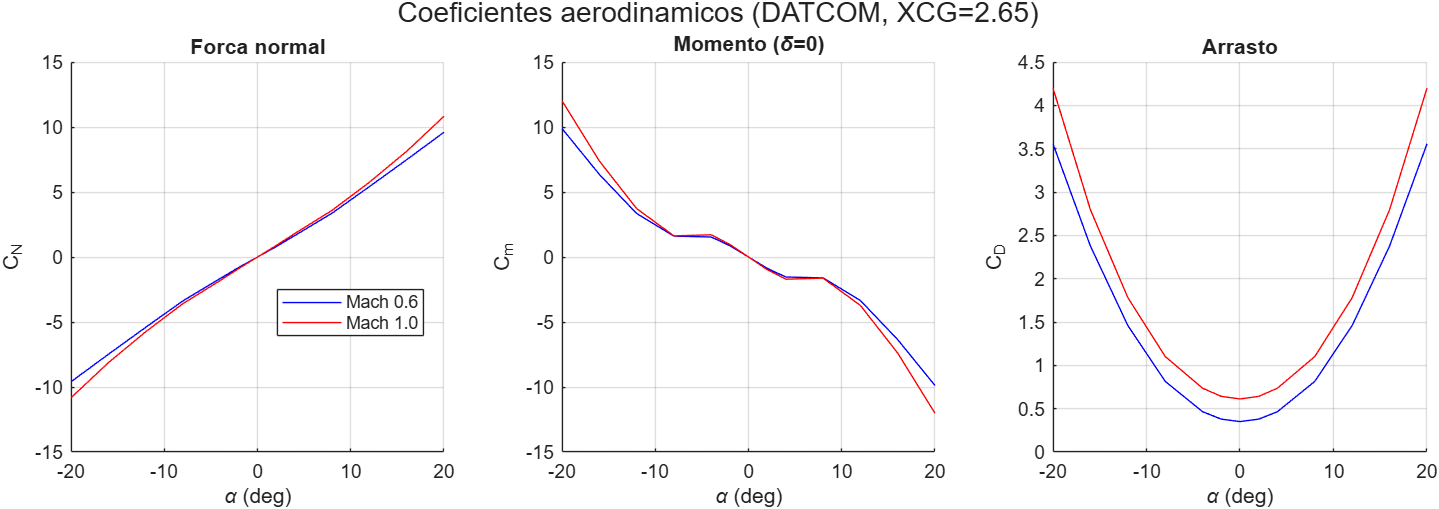
\includegraphics[width=0.86\textwidth]{figures/aero_coef.png}
\caption{Aerodynamic coefficients $C_N$, $C_m$ and $C_D$ versus $\alpha$.}
\end{figure}
